\documentclass[oneside, 11pt]{article}

\usepackage[T1]{fontenc}
\usepackage[utf8]{inputenc}
\usepackage[english]{babel}

\usepackage{fouriernc}
\usepackage[detect-all, binary-units, separate-uncertainty=true,
            per-mode=symbol, retain-explicit-plus, retain-unity-mantissa=false]{siunitx}

\usepackage{setspace}
\setstretch{1.2}

\setlength{\parskip}{\smallskipamount}
\setlength{\parindent}{0pt}

\usepackage[headheight=14pt]{geometry}
\geometry{marginparwidth=0.5cm, verbose, a4paper, tmargin=3cm, bmargin=3cm,
          lmargin=2cm, rmargin=2cm}

\usepackage{float}

\usepackage[fleqn]{amsmath}
\numberwithin{equation}{section}
\numberwithin{figure}{section}

\usepackage{graphicx}
\graphicspath{{images/}{../../../images/}}

\usepackage{tikz}
\usetikzlibrary{shapes}
\usetikzlibrary{plotmarks}

\newcounter{Exercise}
\setcounter{Exercise}{1}
\usepackage{xcolor}
\definecolor{shadecolor}{gray}{0.9}
\usepackage{framed}
\usepackage{caption}

\usepackage{url}


\usepackage{fancyhdr}
\pagestyle{fancy}
\fancyhf{}
\rhead{\thepage}
\renewcommand{\footrulewidth}{0pt}
\renewcommand{\headrulewidth}{0pt}

\fancypagestyle{firststyle}
{
    \fancyhf{}
    \rhead{\thepage}
    \cfoot{
\includegraphics[height=30pt]{HiSPARClogo}}
    \rfoot{
\includegraphics[height=25pt]{CCbysa}}
    \lfoot{
\includegraphics[height=30pt]{NIKHEFlogo}}
    \renewcommand{\footskip}{50pt}
    \renewcommand{\footrulewidth}{0.1pt}
    \renewcommand{\headrulewidth}{0pt}
}

\newcommand{\figref}[1]{Figuur~\ref{#1}}

\newcommand{\hisparc}{\textsmaller{HiSPARC}\xspace}
\newcommand{\kascade}{\textsmaller{KASCADE}\xspace}
\newcommand{\sapphire}{\textsmaller{SAPPHiRE}\xspace}
\newcommand{\jsparc}{\textsmaller{jSparc}\xspace}
\newcommand{\hdf}{\textsmaller{HDF5}\xspace}
\newcommand{\aires}{\textsmaller{AIRES}\xspace}
\newcommand{\csv}{\textsmaller{CSV}\xspace}
\newcommand{\python}{\textsmaller{PYTHON}\xspace}
\newcommand{\corsika}{\textsmaller{CORSIKA}\xspace}
\newcommand{\labview}{\textsmaller{LabVIEW}\xspace}
\newcommand{\daq}{\textsmaller{DAQ}\xspace}
\newcommand{\adc}{\textsmaller{ADC}\xspace}
\newcommand{\hi}{\textsc{h i}\xspace}
\newcommand{\hii}{\textsc{h ii}\xspace}
\newcommand{\mip}{\textsmaller{MIP}\xspace}
\newcommand{\hisparcii}{\textsmaller{HiSPARC II}\xspace}
\newcommand{\hisparciii}{\textsmaller{HiSPARC III}\xspace}

\DeclareSIUnit{\electronvolt}{\ensuremath{\mathrm{e\!\!\:V}}}

\DeclareSIUnit{\unitsigma}{\ensuremath{\sigma}}
\DeclareSIUnit{\mip}{\textsmaller{MIP}}
\DeclareSIUnit{\adc}{\textsmaller{ADC}}

\DeclareSIUnit{\gauss}{G}
\DeclareSIUnit{\parsec}{pc}
\DeclareSIUnit{\year}{yr}




%document details
\author{N.G. Schultheiss \\ translated and adapted by K. Schadenberg}
\date{}
\title{Collisions}


\begin{document}
\maketitle

\section{Introduction}
The world around is us held together by different forces, but these same forces can sometimes be destructive. In this module we will look at what happens when to objects collide with each other. During a collision of two objects (bodies) they exert forces upon each other. These objects can be very large, such as a truck hitting a concrete wall, but also very small, two atoms smashing together. Perhaps chemistry can be seen as the collision and subsequent rearrangement of two or more molecules or atoms.

There are two different types of collisions, elastic and inelastic collisions.
\begin{itemize}
\item During elastic collisions there is no loss of kinetic energy. In reality with almost every collision there is some conversion of energy. For instance, when two snooker balls hit each other you can hear this, this sound is also a form of energy. But in most cases the simplification to a truly elastic collision introduces only a very small error.
\item During inelastic collisions there is a conversion of kinetic energy into other forms of energy. Momentum however is conserved.
\end{itemize}

A further distinction in types of collisions can be made between head-on collisions and oblique or non-head on collisions.\footnote{Non-head on collisions are sometimes called two-dimensional collision because one needs to look at the speed (or energy or momentum) in two dimensions. Some confusion might arise however when using this terminology. Everything drawn in this text is in 2D, it can be quite difficult to draw something to appear to come out of the paper.} 

\section{Conservation Laws}
In physics there are a number of conservation laws. Some are exact while others are approximate. This may already seems strange, a law which is `kind of fuzzy'. However remember that the laws in physics are only true until it has been shown that they can be violated. With the approximate laws we know when they are not valid any more.

An example of an exact law is the conservation of electric charge; the amount of positive charge minus the amount of negative charge in the universe cannot change. Another example is the conservation of (linear) momentum which we will study further in this text.

An examples of an approximate law is the conservation of mass. When there are nuclear reactions or when we approach relativistic speeds mass is not conserved. But in the absence of these processes we can assume a conservation of mass. In particle physics there are a number of approximate laws which tell us what should happen during most particle collisions, but when something extraordinary happens these laws are violated. When and why this happens is the area of much research.

\subsection{Conservation of Linear Momentum}
In a collision a minimum of two objects are involved. A collision of three or more objects at the same time is also possible, but for now we will only look at two. Lets look for instance at a scooter hitting a dustbin. These two object are part of the scooter/dustbin-system. According to Newton's third law, $\textbf{F}_{\begin{tiny}\mbox{action}\end{tiny}}=-\textbf{F}_{\begin{tiny}\mbox{reaction}\end{tiny}}$\footnote{Variables denoted with a \textbf{bold} font are vectors. They have a size (magnitude) and direction. If we are only interested in the size of the force $\textbf{F}_{\begin{tiny}\mbox{action}\end{tiny}}$ we would write $F_{\begin{tiny}\mbox{action}\end{tiny}}$.}, the two bodies exert the same but opposite force upon each other.\footnote{This is not the same as saying that the forces acting upon these bodies are in equilibrium, that would be a special case of Newton's second law.} Before and after the collision this force is 0~N. During the collision, which lasts just as long for both bodies, the forces are not equal to zero any more. In our scooter/dustbin-system the scooter slows down while the dustbin picks up speed.\footnote{We could have said that the scooter decelerated while the dustbin accelerated. In every day speech this is perfectly fine and everybody would understand the meaning. In physics however, we need to be very careful in our wording. Acceleration is the rate at which the velocity of a body changes with time. This change can be an increase or decrease. Deceleration is a negative acceleration. Thus saying that both objects accelerated is a correct use of the word according to physics, but it might raise a few eyebrows if you say it like that to non physicists.} Lets look at these accelerations in a bit more detail using Newton's second law:
\begin{align}
\textbf{F} &= m\textbf{a}  \Longleftrightarrow \label{eq:New2_1} \\
\textbf{F} &= m\frac{\Delta \textbf{v}}{\Delta t} \Longleftrightarrow \label{eq:New2_2} \\
\textbf{F} \Delta t &= m\Delta \textbf{v} = \Delta \textbf{p} \label{eq:New2_3}
\end{align}

Equations~\ref{eq:New2_1}, \ref{eq:New2_2}, and \ref{eq:New2_3} are three different ways of writing the same law. When describing collisions and performing calculations on them the last notation is most frequently used. It describes the change in momentum (\textbf{p}). Because the forces acting upon the scooter and dustbin are of equal size, the change in momentum must also be the same for both objects. But the forces were in opposite directions, so the change in momentum must also be in opposite direction. This brings us to the law of conservation of momentum. The sum of the momenta of all objects before and after a collision must be the same:
\begin{equation}
\sum \textbf{p} = \mbox{constant}
\end{equation}

In classical physics (machanics) the momentum is calculated as follows:
\begin{equation}
\textbf{p}=m\textbf{v}
\end{equation}

\section{Conservation of Energy}
A second property/quantity which is conserved in nature is energy. Energy can be converted from one form to another, e.g. a ball dropping from a height transforms it potential gravitational energy into kinetic energy, but energy cannot disappear or be created.

We will first look at elastic collisions in which there is no conversion of energy. In the previous section we saw that the collision time for both objects is the same. During that time the point of contact between the two object might move. To calculate the transfer of (kinetic) energy from object I (e.g. the scooter) to object II (e.g. the dustbin) we calculate the work done by object I.\footnote{Our scooter might belong to a pizza delivery boy who, while working hard, hits a dustbin. In physics however, only forces can do work.}
\begin{equation}
W=\textbf{F}s
\end{equation}
In our system of two bodies:
\begin{equation}
\left\lbrace  \begin{array}{rl}
W_I &= \textbf{F}_I \textbf{s} \\
W_{II} &= \textbf{F}_{II} \textbf{s} \\
-\textbf{F}_I &= \textbf{F}_{II} \end{array} \Rightarrow \right\rbrace -W_I = W_{II}
\end{equation}
Because object I, by doing work, supplies the same amount of energy as being received by object II, we can say that the total amount of energy remains constant. The law of conservation of energy is therefore valid for elastic collisions.
\begin{equation}
\sum E =\mbox{constant}
\end{equation}

Lets use the equations above to calculate what exactly happens during the collision between the scooter and the dustbin. Our scooter, object I, has a mass of 60~kg. It hits the stationary dustbin, object II, which has a mass of 30~kg, with a speed of 10~m/s. We can write this and the solution to our problem down in a concise and organised manner:

\subsubsection*{Given before collision:}
\begin{itemize}
\item[-] $v_I = 10$~m/s
\item[-] $m_I = 60$~kg
\item[-] $v_{II} = 0$~m/s
\item[-] $m_{II} = 30$~kg
\end{itemize}

\subsubsection*{Wanted:}
\begin{itemize}
\item[-] The speeds after collision.
\end{itemize}

\subsubsection*{Equations:}
\begin{itemize}
\item[-] $E_{\begin{tiny}\mbox{kin}\end{tiny}}=\frac{1}{2}mv^2$
\item[-] $\textbf{p}=m\textbf{v}$
\end{itemize}

\subsubsection*{Solution:}
\begin{doublespace}
Energy during/after collision $E_{\begin{tiny}\mbox{system}\end{tiny}}=\frac{1}{2}m_I v_I^2 + \frac{1}{2}m_{II} v_{II}^2$\\
or before collision $E_{\begin{tiny}\mbox{system}\end{tiny}}=\frac{1}{2}m_I v_I^2 + \frac{1}{2}m_{II} v_{II}^2 =\frac{1}{2} \cdot 60~\mbox{kg} \cdot (10~\mbox{m/s})^2 + \frac{1}{2} \cdot 30~\mbox{kg} \cdot (0~\mbox{m/s})^2 = 3000~\mbox{J}$\\
Momentum during/after collision $p=m_I v_I + m_{II} v_{II}$\\
or before collision $p=60~\mbox{kg} \cdot 10~\mbox{m/s} + 30~\mbox{kg} \cdot 0~\mbox{m/s} = 600~\frac{\mbox{kgm}}{\mbox{s}}$\\ \\
Momentum after collision $p=60~\mbox{kg} \cdot v_I + 30~\mbox{kg} \cdot v_{II} = 600~\frac{\mbox{kgm}}{\mbox{s}} \Longrightarrow v_{II} = 20~\mbox{m/s} - 2v_I$  \\
Substitution yields $E_{\begin{tiny}\mbox{system}\end{tiny}}=\frac{1}{2} \cdot 60~\mbox{kg} \cdot v_I^2 + \frac{1}{2} \cdot 30~\mbox{kg} \cdot (20~\mbox{m/s} - 2v_I)^2 = 3000~\mbox{J}$\\
Solving this quadratic equation\footnote{Use the quadratic formula to solve this equation.} yields two answers: $v_I=10~\mbox{m/s}$ and $v_I=3.3~\mbox{m/s}$\\
The first solution is the situation before the collision, the second after the collision. The speed of the dustbin after the collision is therefore: $v_{II}=20~\mbox{m/s} - 2v_{I}=13.3~\mbox{m/s}$
\end{doublespace}

Suppose the scooter lies stationary on the ground after the collision with the dustbin. Can we now calculate how much energy has been transformed into heat? Of course we must not forget the law of conservation of momentum. Because the scooter is now stationary the entire momentum of the system must now held by the dustbin. Calculating the speed of the dustbin in this case is easy. The mass of the dustbin is half that of the scooter, its speed after the collision is therefore double that of the scooter before the collision, i.e. $20~\mbox{m/s}$. This would mean that the energy of the dustbin is 6000~J after the collision, more than the 3000~J that was present before the collision. The only possible conclusion is that this kind of collision is not possible because it violates the law of conservation of energy.


\begin{shaded}
\textbf{Exercise \theExercise \stepcounter{Exercise}} : Calculate how much energy in transformed from kinetic energy into a different kind of energy (such as heat or sound) when the scooter has a speed of $5~\mbox{m/s}$ after the collision.\end{shaded}
\begin{shaded}
\textbf{Exercise \theExercise \stepcounter{Exercise}} : Suppose the scooter and dustbin `stick together' after the collision. How much energy is transformed in this situation? \end{shaded}

\section{Oblique Collisions}
Collisions need not be head-on. In the previous section assumed as much when the scooter hit the dustbin, but what happens when the scooter hits the dustbin at an angle?

As an example of a two-dimensional collision we will look at a `simple' snooker play. With simple we mean that the balls are played without any spin. Take a look at figure~\ref{fig:snooker1}, to pot the black ball, a simple head-on collision will not suffice. We need to look `over' the black ball at the pocket to see where we need to hit it with the cue ball. The cue ball needs to hit the black ball on the extension of the line between the black ball and the pocket. At the moment of collision the line between the centres of the balls points towards the pocket. 

\begin{figure}\begin{center}
\begin{picture}(0,0)%
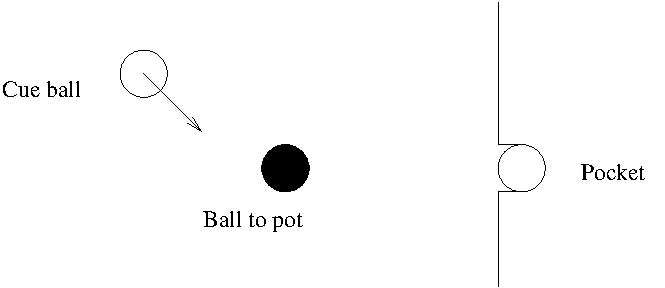
\includegraphics{snooker1}%
\end{picture}%
\setlength{\unitlength}{4144sp}%
%
\begingroup\makeatletter\ifx\SetFigFont\undefined%
\gdef\SetFigFont#1#2#3#4#5{%
  \reset@font\fontsize{#1}{#2pt}%
  \fontfamily{#3}\fontseries{#4}\fontshape{#5}%
  \selectfont}%
\fi\endgroup%
\begin{picture}(5055,2184)(706,-4123)
\end{picture}%
\caption{Snooker table before collision.}\label{fig:snooker1}
\end{center}\end{figure}

How do we solve this problem? We can decompose all velocities and momenta into vectors; into the x and y direction. A logical choice of the x and y direction would be two perpendicular sides of the table. But we can also choose to `attach' the y-axis to the cue ball. In this axis (or coordinate) system figure~\ref{fig:snooker1} transforms into \ref{fig:snooker2}. Now the cue ball only has a speed in the x direction but both the black ball and pocket are moving upwards.

\begin{figure}[h]\begin{center}
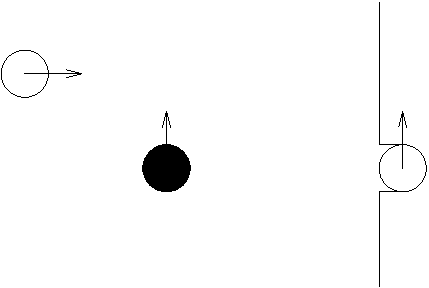
\includegraphics{snooker2}%
\caption{Figure~\ref{fig:snooker1} in the new coordinate system.}\label{fig:snooker2}
\end{center}\end{figure}

We want to hit the black ball as drawn in figure~\ref{fig:snooker3}, head-on, to pot it. 
\begin{shaded}
\textbf{Exercise \theExercise \stepcounter{Exercise}} : Both balls have the same mass. Show that the cue ball transfers all its momentum to the black ball.\\
Hint: You only need to look at the momentum in the x-direction. What is the speed of the black ball in the x-direction?
\end{shaded}

\begin{figure}\begin{center}
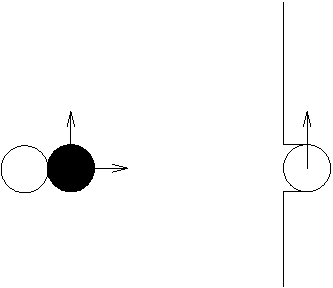
\includegraphics{snooker3}%
\caption{Collision in the new coordinate system.}\label{fig:snooker3}
\end{center}\end{figure}

The situation after the collision is as drawn in figure~\ref{fig:snooker3}. How does this look from the players point of view? We reattach the coordinate system to the table and obtain figure~\ref{fig:snooker4}. The cue ball is moving in the negative y direction, the pocket is stationary again, and the black ball is moving towards the pocket. 

\begin{figure}\begin{center}
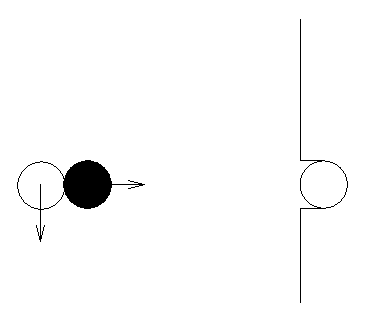
\includegraphics{snooker4}%
\caption{Figure~\ref{fig:snooker3} in the original coordinate system of figure~\ref{fig:snooker4}.}\label{fig:snooker4}
\end{center}\end{figure}

Using the above `trick' of transforming the coordinate system two times we can solve our non-head-on collision.

\end{document}


\begin{shaded}
\textbf{Exercise \theExercise \stepcounter{Exercise}} : \end{shaded}

\footnotemark
\footnotetext{}
